
% Szkielet dla pracy pisanej w języku polskim.

\documentclass[polish,a4paper,oneside]{ppfcmthesis}


\usepackage[utf8]{inputenc}
\usepackage[OT4]{fontenc}


\author{Ignacy Iksiński}                              % Your name comes here
\title{W zdrowym ciele zdrowy~duch}                   % Note how we protect the final title phrase from breaking
\ppsupervisor{prof.~dr hab.~inż.~Alojzy Wołodyjowski} % Your supervisor comes here.
\ppyear{2006}                                         % Year of final submission (not graduation!)


\begin{document}

% Front matter starts here
\frontmatter\pagestyle{empty}%
\maketitle\cleardoublepage%

% Blank info page for "karta dyplomowa"
\thispagestyle{empty}\vspace*{\fill}%
\begin{center}Tutaj przychodzi karta pracy dyplomowej;\\oryginał wstawiamy do wersji dla archiwum PP, w pozostałych kopiach wstawiamy ksero.\end{center}%
\vfill\cleardoublepage%

% Table of contents.
\pagenumbering{Roman}\pagestyle{ppfcmthesis}%
\tableofcontents* \cleardoublepage%

% Main content of your thesis starts here.
\mainmatter%

\chapter{Wstęp}
Realizacja niniejszej pracy inżynierskiej została rozpoczęta w~grudniu 2005 roku
jako projekt w~konkursie
\akronim{\htmladdnormallink{CSIDC}{http://computer.org/csidc}}
(\english{Computer Society International Design Competition}). Organizatorem
konkursu jest Towarzystwo Komputerowe przy amerykańskim Instytucie Inżynierii
Elektrotechnicznej i~Elektronicznej (\english{IEEE Computer Society}). Konkurs
ten zachęca studentów do pracy w~zespole w~celu stworzenia opartego na
wykorzystaniu komputerów rozwiązania dla wybranego problemu. Zadaniem studentów
jest zaprojektowanie, wykonanie, przetestowanie, udokumentowanie, a~nawet
sprzedanie wynalezionego przez nich systemu. Konkurs rozgrywany jest w~trzech
etapach. W~pierwszym etapie studenci analizują zadany temat, wybierają problem i
zgłaszają temat pracy. Ze wszystkich zgłoszeń wybieranych jest 300 drużyn, które
przystępują do zgłębienia problemu i~przygotowują plan realizacji projektu.
Rezultatem jest raport wstępny (\english{Interim Report}), na podstawie którego
100 najlepszych drużyn kwalifikuje się do trzeciego etapu. Następnie zespoły te
realizują zaplanowane prace i~przygotowują raport finałowy (\english{Final
Report}). Autorzy dziesięciu najlepszych prac są zapraszani na finały do
Waszyngtonu, D.C., gdzie zespoły prezentują swoje projekty. Na podstawie
prezentacji i~raportu finałowego wybierani są zwycięzcy konkursu. Temat
\akronim{CSIDC} w~2006 roku brzmiał: ,,Preserving, Protecting and Enhancing the
Environment'', czyli w~wolnym tłumaczeniu ,,Podtrzymywanie, Ochrona i~Ulepszanie
Środowiska''. Niniejszy projekt został zakwalifikowany do III etapu konkursu,
a~następnie był rozwijany i~doczekał się obecnej formy pracy inżynierskiej.

Szeroko pojęta ochrona środowiska kojarzona jest zazwyczaj z~zanieczyszczeniami
środowiska (powietrza, wody lub gleby) czy globalnym ociepleniem. Do kwestii
wymierania gatunków przywiązuje się wagę dużo mniejszą, podczas gdy niezmiernie
istotne jest to, że spośród wielu codziennie wymierających gatunków każdy
ewoluował do obecnej postaci miliony lat i~ma wielki wpływ na równowagę swojego
ekosystemu. Pomoc w~przetrwaniu chociaż jednego gatunku wnosi istotny wkład
w~ochronę środowiska.

Inspiracją do napisania niniejszej pracy były rozmowy z~pracownikami Poznańskiego
Nowego Zoo. Dyrektor do spraw hodowli tego ogrodu, dr~inż.~Radosław Ratajszczak,
opowiedział o~następujących wydarzeniach:
\begin{quote}
	 W~1974 roku światowa populacja jednej z~odmian pustułki (łac. \emph{mauritius
	 kestrel}) liczyła 10~sztuk, wśród których były tylko 2~samice. Wszystkie
	 ptaki żyły w~niewoli -- gatunek był bardzo bliski wymarcia. Minęły dwa lata
	 zanim jedna z~samic złożyła jedno jajo. Zostało ono wzięte do inkubatora, by
	 zapewnić mu przetrwanie. Inkubacja się udała, pisklę się wykluło, ale
	 wydarzył się straszny wypadek: eter, który był używany w~czujniku inkubatora
	 wyciekł i~zatruł pisklę. Jak widać, bezsensowny wypadek o~mały włos nie
	 doprowadził do wyginięcia gatunku.
\end{quote}
Na szczęście pustułki nie wymarły, a~ich dzisiejsza populacja oceniana jest
na~ok.~150 sztuk. Mimo to ta historia powinna być traktowana jako
ostrzeżenie, bo podobny wypadek w~przyszłości może mieć fatalne konsekwencje.

Inkubacja zagrożonych gatunków jest bardzo trudnym zadaniem i~wymaga
odpowiednich narzędzi. Analiza problemu wykazała że~istniejące inkubatory
zapewniają tylko podstawową funkcjonalność, niewystarczającą dla wielu
gatunków, a~także że brakuje inkubatorów ułatwiających prowadzenie badań
naukowych. Podstawowa funkcjonalność której oczekują ornitolodzy to możliwość
analizy przebiegu inkubacji (zapisywanie stanu inkubatora i~możliwość jego
wizualizacji) czy też programowalność (możliwość zaprogramowania zmiany
parametrów inkubacji w~czasie). Dodatkowo pożądana była możliwość zbierania
i~analizowania danych z~wielu inkubatorów.

Powyższe przemyślenia zainspirowały autorów niniejszej pracy do stworzenia
Thinkubatora -- systemu umożliwiającego inkubację ptasich jaj w~kontrolowanym
i~nadzorowanym środowisku, który może zrewolucjonizować podejście do inkubacji.
W~centrum systemu znajduje się wysokiej jakości inkubator. Jest on wyposażony
w~komputer przemysłowy z~interfejsem ethernetowym umożliwiającym komunikację ze
Stacją Kontrolną -- aplikacją zainstalowaną na~komputerze klasy PC umożliwiającą
bezpośrednią interakcję z~inkubatorami. Za pomocą Stacji Kontrolnej można
programować i~nadzorować wiele inkubatorów -- oszczędza się dzięki temu czas
potrzebny na programowanie wielu urządzeń. Stacja Kontrolna umożliwia także
zapisywanie informacji o~stanie inkubacji w~celu ich wizualizacji lub do
późniejszej analizy. Cały system jest zintegrowany ze zdalnym serwerem --
Centrum Nadzoru. Serwer zbiera dane z~wszystkich inkubatorów umożliwiając
zaawansowaną analizę statystyczną lub analizę przy pomocy algorytmów wspomagania
decyzji. Umożliwia on także wymianę informacji pomiędzy użytkownikami na całym
świecie. Posiada również funkcję wizualizacji danych, która pozwala na
współdzielenie wiedzy o~ptakach pomiędzy profesjonalistami a~hobbistami i~jej
poszerzanie.

Ornitolodzy z~Zoo w~Poznaniu uważają, że system o~takich parametrach jest
wysoce pożądany. Analiza kosztów, zalet i~wad tego systemu pokazała, że mógłby
on zostać bez problemu wdrożony w~wielu ogrodach zoologicznych na świecie.

Pomimo dużej funkcjonalności i~zastosowania wielu przydatnych rozwiązań koszt
urządzenia wraz z~wdrożeniem byłby niższy niż koszt wdrożenia zwykłego
inkubatora o~podobnych parametrach.

W realizacji projektu brały udział cztery osoby. Tabela \ref{tab:Podzial}
przedstawia zadania wykonane przez każdą z nich.

Struktura pracy jest następująca. W~rozdziale~\ref{sec:CeliZakres} opisano
obecny stan wiedzy na temat inkubacji ptasich jaj, stosowane rozwiązania
w~komercyjnych inkubatorach oraz dokładnie zdefiniowano cel projektu.
W~rozdziale~\ref{sec:Architektura} opisano architekturę systemu Thinkubator.
Jest on podzielony na cztery podrozdziały, opisujące realizację poszczególnych
elementów systemu oraz zastosowane metody komunikacji między nimi.
W~rozdziale~\ref{sec:Praktyka} opisano przykładowy scenariusz użycia systemu
wraz z~krókim opisem interfejsu użytkownika. Praca zakończona jest krótkim
podsumowaniem w~rozdziale~\ref{sec:Podsumowanie}.

\begin{table}[b]
	\centering
	\begin{tabular}{|m{6cm}|c|c|c|c|}\hline
		\bfseries Czynność & \bfseries Janusz & \bfseries Paweł & \bfseries Tomasz &
		\bfseries Szymon \\
		& \bfseries Bossy & \bfseries Lubarski & \bfseries Nowak & \bfseries
		Szafraniec \\\hline
		\multicolumn{5}{|c|}{\bfseries Budowa inkubatora} \\\hline
		Wysokopoziomowy projekt inkubatora & $\checkmark$ & $\checkmark$ &
		$\checkmark$ & $\checkmark$ \\\hline
		Projekt wymiennika ciepła & $\checkmark$ & $\checkmark$ & $\checkmark$ &
		$\checkmark$ \\\hline
		Wykonanie wymiennika ciepła & $\checkmark$ & $\checkmark$ & & $\checkmark$
		\\\hline
		Wykonanie konstrukcji zewnętrznej & $\checkmark$ & $\checkmark$ & &
		$\checkmark$ \\\hline
		Projekt komory inkubacyjnej & $\checkmark$ & $\checkmark$ & & $\checkmark$
		\\\hline
		Montaż elektroniki & $\checkmark$ & $\checkmark$ & $\checkmark$ &
		$\checkmark$ \\\hline 
		Wykonanie elektroniki peryferyjnej & & & $\checkmark$ & \\\hline
		Montaż inkubatora & $\checkmark$ & $\checkmark$ & $\checkmark$ &
		$\checkmark$ \\\hline 
		\multicolumn{5}{|c|}{\bfseries Oprogramowanie inkubatora} \\\hline
		Projekt wysokopoziomowy & $\checkmark$ & $\checkmark$ & $\checkmark$ &
		$\checkmark$ \\\hline 
		Implementacja jądra systemu & $\checkmark$ & & & \\\hline
		Projekt algorytmów sterowania & $\checkmark$ & $\checkmark$ & & $\checkmark$
		\\\hline
		Implementacja algorytmów sterowania & $\checkmark$ & $\checkmark$ & &
		$\checkmark$ \\\hline
		Kalibracja algorytmów sterowania & $\checkmark$ & $\checkmark$ & &
		$\checkmark$ \\\hline
		Oprogramowanie UI & & & $\checkmark$ & \\\hline
		Uruchomienie \emph{SBC} & $\checkmark$ & $\checkmark$ & $\checkmark$ &
		$\checkmark$ \\\hline
		Implementacja algorytmów komunikacji & $\checkmark$ & $\checkmark$ & & $\checkmark$
		\\\hline
		\multicolumn{5}{|c|}{\bfseries Stacja Kontrolna} \\\hline
		Projekt wysokopoziomowy & $\checkmark$ & $\checkmark$ & & $\checkmark$
		\\\hline
		Implementacja & $\checkmark$ & & & $\checkmark$ \\\hline
		Implementacja algorytmów komunikacji & $\checkmark$ & & & $\checkmark$
		\\\hline
		\multicolumn{5}{|c|}{\bfseries Centrum Nadzoru} \\\hline
		Projekt wysokopoziomowy &		$\checkmark$ & $\checkmark$ & & $\checkmark$
		\\\hline
		Implementacja UI & & $\checkmark$ & & \\\hline
		Projekt schematu bazy danych & $\checkmark$ & $\checkmark$ & & $\checkmark$
		\\\hline
		Implementacja algorytmów komunikacji & & $\checkmark$ & & \\\hline
	\end{tabular}
	\caption{Podział prac}
	\label{tab:Podzial}
\end{table}

\section{Stosowane rozwiązania}
W trakcie realizacji projektu Poznańskie Nowe Zoo dysponowało kilkoma
inkubatorami, pozwalającymi na inkubację łącznie około 200 jaj o~rozmiarach od
pustułczych do strusich. Urządzenia te zostały zakupione w~przeciągu ostatnich
20 lat i~stosują wiele nieaktualnych rozwiązań, posiadają liczne wady
i~ograniczenia. Stosują one sterowanie liniowe. Zadane wartości \emph{sterowanych
parametrów} (temperatury, wilgotności, częstości obracania jaj) ustawia się
w~nich przy pomocy pary analogowych pokręteł, co jest nieprecyzyjne. Co więcej,
pokrętła są podatne na przypadkowe zmiany pozycji i~trudno jest z~nich odczytać
faktycznie nastawione wartości. Absurdalną sytuację zaobserwowano, gdy
pracownicy Zoo kreślili po obudowie inkubatora, aby zapamiętać jakie powinny być
położenia pokręteł. Aktualną temperaturę w~stosowanych
inkubatorach można zweryfikować jedynie poprzez odczytanie wskazania rtęciowego
termometru umieszczonego wewnątrz inkubatora. Analogowe metody pomiarów
i~sterowania są niedoskonałe i~podatne na wzrost błędu wraz z~czasem życia
urządzenia. Niektóre inkubatory wymagały też regularnej interwencji personelu
w~celu obrócenia jaj.

Nowoczesne inkubatory \cite{Brinsea} \cite{Metzer} rozwiązują część z~powyższych problemów. Posiadają takie
cechy jak elektroniczne sterowanie temperaturą, wilgotnością i~wentylacją oraz
niezależne cyfrowe termometry gwarantujące obiektywny odczyt. Niektóre
rozwiązania wyposażone są w~alarm informujący o~zbyt wysokiej lub zbyt niskiej
temperaturze czy też awarii zasilania, a~także posiadają w~pełni automatyczny
mechanizm obracania jaj, poprzez rotację komory inkubacyjnej.

Mimo postępu technologii zarówno w~starszych inkubatorach jak i~w urządzeniach najnowszych programowanie działania inkubatora ogranicza się do zadania stałej wartości
sterowanym parametrom. Tymczasem możliwość zaprogramowania zmiennej w~czasie
funkcji temperatury lub wilgotności jest bardzo pożądana przez ornitologów.
Podczas inkubacji niektórych gatunków co kilka dni trzeba zmieniać ręcznie
ustawienia temperatury i~wilgotności. Ponadto w~celu symulowania warunków
naturalnych co kilka godzin wietrzy się inkubatory na kilkanaście minut.
%[[ symulując sytuację, gdy wysiadujący ptak schodzi z~jaj. ]]
W~istniejących rozwiązaniach brakuje też możliwości rejestracji przebiegu
inkubacji. Aby upewnić się, że urządzenie w~danej chwili działa prawidłowo,
ornitolog musi odczytać wartości sterowanych parametrów bezpośrednio
z~inkubatora. W~przypadku nieudanej inkubacji, czyli niskiej klujności zdrowych
zalążków, niemożliwa jest ocena przyczyn niepowodzenia. W~szczególności, nie
można powiedzieć, czy zawiniły błędy teoretyczne, czyli niewłaściwie dobrane
wartości sterowanych parametrów, czy błędy techniczne, jak np. nocna awaria
zasilania. Te ograniczenia znacznie utrudniają prowadzenie badań naukowych na
temat inkubacji.

Projekt Thinkubator ma za zadanie wprowadzić nową jakość do procesu inkubacji.
Ma on umożliwiać programowanie dowolnej zmienności wszystkich sterowanych
parametrów inkubacji w~czasie. W~prosty sposób da możliwość nastawienia chłodzenia,
dobowych wahań temperatury oraz automatycznego rolowania. Po zaprogramowaniu
inkubatora system będzie nieustannie monitorować proces inkubacji, co będzie umożliwiać
sprawdzenie przebiegu procesu zarówno w~trakcie jego trwania jak i~po jego
zakończeniu. Dzięki temu będzie to jedyny system, który w~takim stopniu wspiera
badania naukowe nad inkubacją zagrożonych gatunków. Dodatkowo system umożliwi
zdalny monitoring inkubatora przez Internet oraz stworzenie mechanizmu szybkich
powiadomień w~przypadku awarii zasilania lub innych niepożądanych zdarzeń.
Będzie pozwalać na współdzielenie doświadczeń z~innymi jego użytkownikami, przez co
umożliwi nawiązywanie współpracy ornitologom z~różnych ogrodów zoologicznych. Ze
współdzielenia informacji będą mogli korzystać również ornitolodzy-amatorzy,
ponieważ narzędzie do programowania inkubacji zaproponuje użytkownikowi
optymalne wartości sterowanych parametrów, nawet przy jednoczesnej inkubacji jaj
różnych gatunków.

\section{Cel projektu}
Celem projektu jest stworzenie systemu do inkubacji jaj ptasich w~kontrolowanym
środowisku. System ten składa z~urządzenia pozwalającego na inkubację jaj
w~warunkach identycznych z~naturalnymi oraz podsystemu informatycznego,
odpowiedzialnego za kontrolę i~analizę procesu inkubacji. Ogólny schemat
połączeń między urządzeniami został przedstawiony na rysunku
\ref{rys:SystemDiagram}.

\subsection{Wizja systemu}
Urządzenia wchodzące w~skład systemu Thinkubator podzielone są na trzy poziomy:

\begin{figure}[t] 
\centering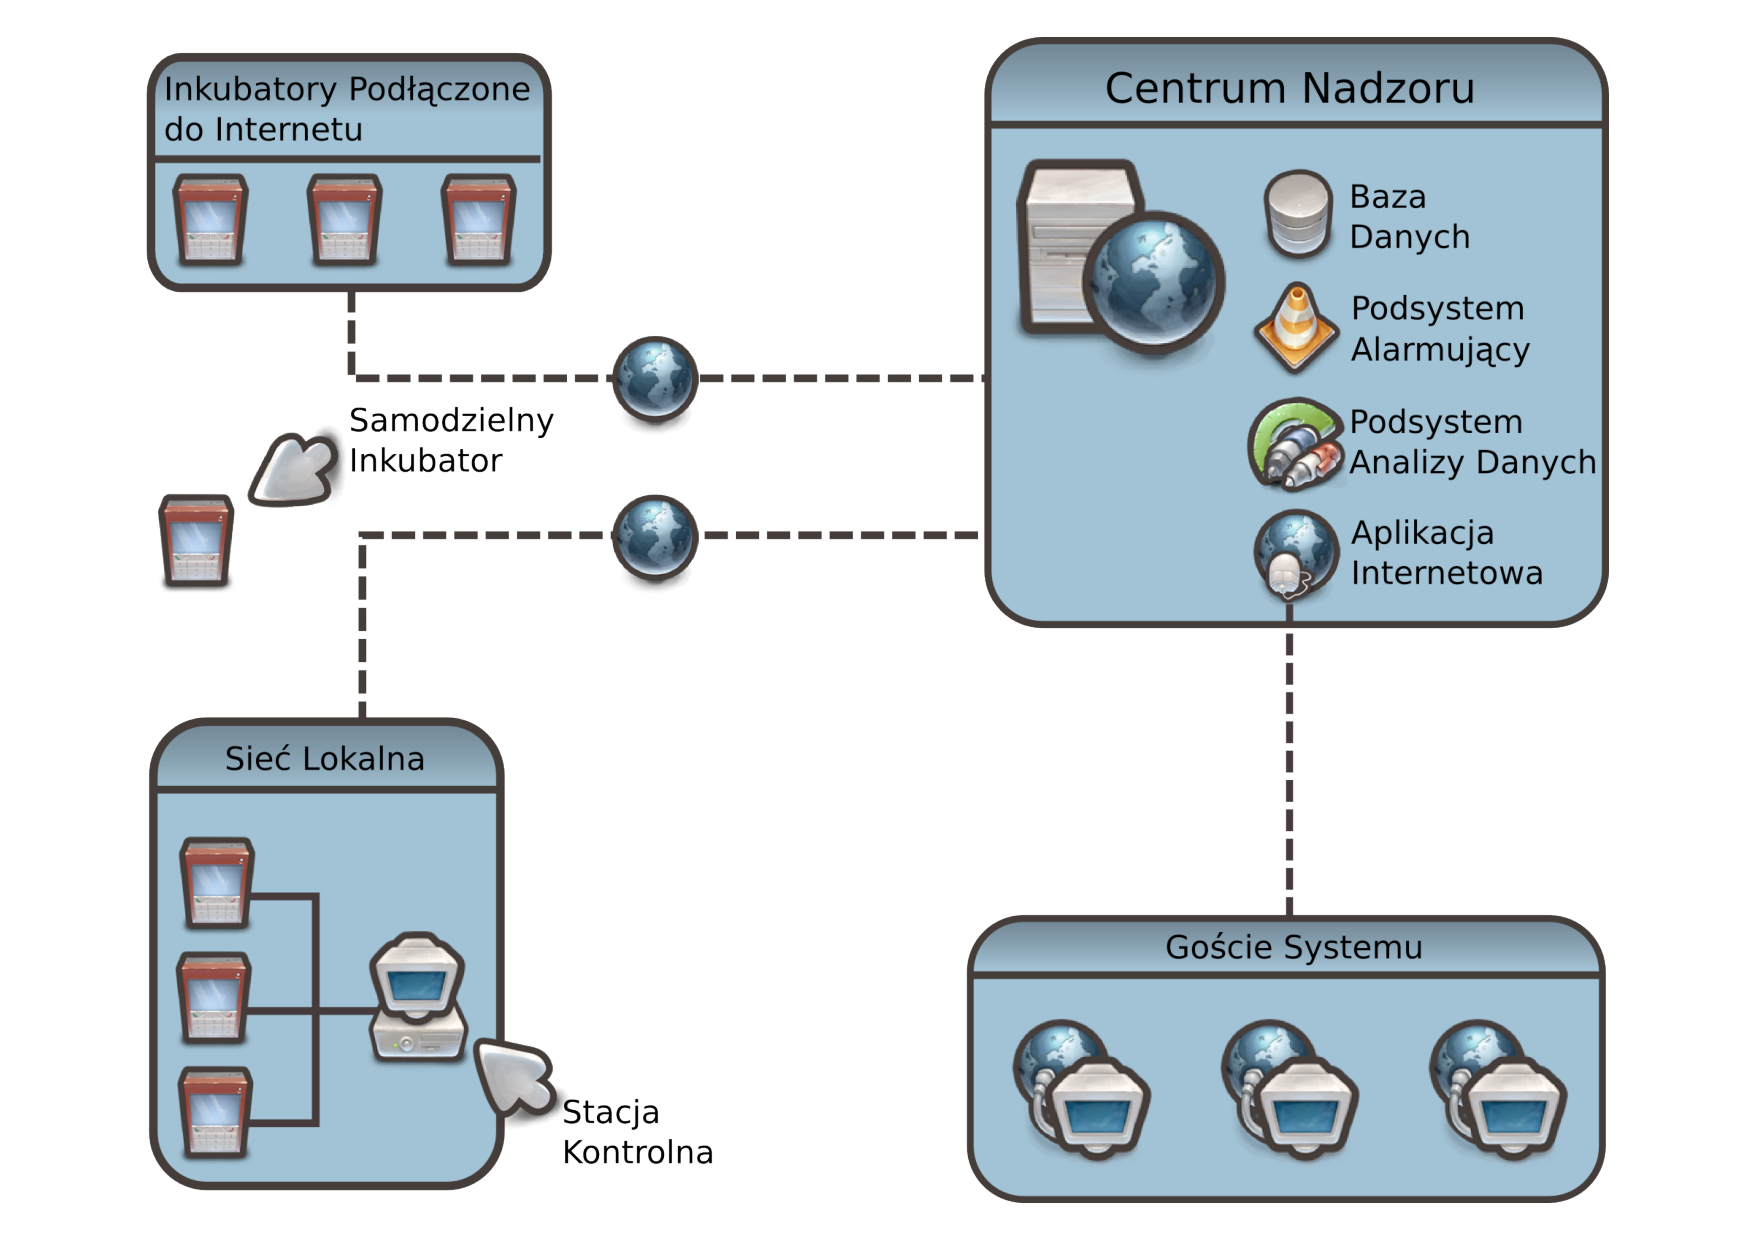
\includegraphics[width=\textwidth]{figures/System_Diagram}
\caption{Diagram systemu}\label{rys:SystemDiagram}
\end{figure}

\paragraph{Poziom 1. -- Inkubator.}
Najważniejszy element systemu. Pozwala na inkubację jaj oraz monitorowanie
tego procesu. Jako samodzielnie urządzenie posiada pełną funkcjonalność typowego
inkubatora. Dodatkowo wyposażony jest w~klawiaturę oraz wyświetlacz LCD,
pozwalające w~intuicyjny sposób programować inkubator oraz wyświetlać aktualne
wartości sterowanych parametrów.

\paragraph{Poziom 2. -- Stacja Kontrolna.}
Komputer połączony z~inkubatorami siecią lokalną Ethernet. Pozwala ornitologom
na zaprogramowanie inkubatora. Pomaga w~doborze optymalnych wartości sterowanych
parametrów w~przypadku jednoczesnej inkubacji jaj różnych gatunków. Na bieżąco
monitoruje i~wizualizuje parametry trwających oraz zakończonych inkubacji.

\paragraph{Poziom 3. -- Centrum Nadzoru.}
Zdalny serwer pracujący non-stop. Składa się z~następujących podsystemów:
\begin{itemize}
	\item bazy danych, która gromadzi informacje o~przebiegu oraz efektywności
		inkubacji ze wszystkich zarejestrowanych w~systemie inkubatorów oraz
		przechowuje wyniki analizy danych,
	\item podsystem alarmowania -- w~równych odstępach czasu rejestruje stan
		wszystkich inkubatorów, a~w~przypadku wykrycia błędnego stanu podejmuje
		odpowiednie działania alarmujące,
	\item podsystem analizy danych -- narzędzia do analizy wpływu warunków
		inkubacji (np. średniej temperatury, najdłuższego czasu bez zasilania) na
		klujność; funkcjonalność ta została zaprojektowana z~myślą o~rozszerzeniu systemu w~przyszłości,
	\item podsystem wizualizacji -- aplikacja internetowa służąca do nadzoru
		systemu i~wizualizacji przechowywanych danych,
	\item podsystem administracyjny -- panel służący do zarządzania inkubatorami.
\end{itemize}

Poszczególne elementy systemu zostały tak zaprojektowane by ściśle
współpracowały z~urządzeniami na niższym poziomie, natomiast były niezależne od
urządzeń na wyższym poziomie. Pozwala to na poprawne działanie systemu
w~przypadku gdy jest on ograniczony do dwóch poziomów (Inkubator i~Stacja
Kontrolna, Inkubator i~Centrum Nadzoru) lub tylko jednego poziomu (Inkubator).
Dodatkowo uniezależnienie poziomów pozwala na zwiększenie niezawodności
systemu oraz zapewnia odporność na utratę danych w~wyniku awarii urządzenia na
niższym poziomie.

\subsection{Zasady działania systemu}
Poniższy scenariusz opisuje ogólny sposób wykorzystania systemu:
\begin{itemize}
	\item Proces inkubacji rozpoczynany jest poprzez umieszczenie w~inkubatorze
		jaj i~zaprogramowanie inkubatora przy pomocy wbudowanej klawiatury lub
		Stacji Kontrolnej. Inkubacja trwa od dwóch tygodni do dwóch miesięcy.
		W~dowolnej chwili można zmienić ustawiony program inkubacji.
	\item Przy programowaniu inkubatora Stacja Kontrolna wyświetla dostępne wzorce
		inkubacji pomagając w~optymalnym doborze sterowanych parametrów.
	\item Stacja Kontrolna regularnie pobiera uaktualnienia wzorców inkubacji
		w~Centrum Nadzoru.
	\item Wartości wszystkich sterowanych parametrów inkubacji są przechowywane
		w~pamięci inkubatora i~mogą być odczytane przez Stację Kontrolną.
	\item Wiadomości kontrolne z~wartościami sterowanych parametrów są wysyłane do
		Stacji Kontrolnej i~Centrum Nadzoru w~równych odstępach czasu.
	\item Ornitolog może sprawdzić stan procesu inkubacji na trzy sposoby (trzy
		poziomy kontroli):
		\begin{itemize}
			\item odczytując wskazania na cyfrowym wyświetlaczu inkubatora,
			\item przy pomocy Stacji Kontrolnej, która wyświetla bieżące wartości
				sterowanych parametrów dla wszystkich działających inkubatorów w~sieci
				lokalnej,
			\item po zalogowaniu do Centrum Nadzoru, do którego ma dostęp z~każdego
				miejsca na świecie.
		\end{itemize}
	\item W~przypadku błędnego stanu inkubacji uruchamiane są trzy sposoby
		alarmowania odpowiadające poziomom kontroli:
		\begin{itemize}
			\item Inkubator -- alarm dźwiękowy,
			\item Stacja Kontrolna -- wyświetlenie powiadomienia,
			\item Centrum Nadzoru -- powiadomienie e-mailowe, możliwość dodania
				funkcjonalności powiadomień sms-owych.
		\end{itemize}
	\item Centrum Nadzoru gromadzi informacje o~przebiegach inkubacji w~celu
		współdzielenia doświadczeń i~analizy danych.
	\item Za przyzwoleniem ogrodu zoologicznego informacja o~stanie inkubatora
		może być udostępniona anonimowym użytkownikom aplikacji internetowej
		w~Centrum Nadzoru. Pozwoli to na zwiększenie zainteresowania użytkowników
		Internetu pracami prowadzonymi w~zoo i~zachęci ich do odwiedzenia ogrodu.
\end{itemize}

\subsection{Opis funkcjonalności systemu}
Poszczególne części systemu thinkubator pełnią następujące funkcje:

\noindent\textbf{Inkubator}:
\begin{itemize}
	\item zapewnienie optymalnych warunków inkubacji poprzez jak najwierniejsze
		odtworzenie rzeczywistych warunków inkubacji,
	\item sterowanie w~zakresie temperatury, wilgotności i~obracania jaj,
	\item wyświetlanie na wyświetlaczu LCD parametrów inkubacji,
	\item możliwość zaprogramowania inkubacji przy pomocy wbudowanej klawiatury,
	\item możliwość zaprogramowania inkubacji przy pomocy Stacji Kontrolnej,
	\item zbieranie danych pomiarowych,
	\item rozsyłanie danych pomiarowych do Stacji Kontrolnej i~Centrum Nadzoru.
\end{itemize}
\textbf{Stacja Kontrolna}:
\begin{itemize}
	\item jednoczesne monitorowanie wszystkich inkubatorów w~sieci,
	\item wizualizacja przebiegu sterowanych parametrów inkubacji w~funkcji czasu
		przez cały okres inkubacji,
	\item programowanie inkubatora,
	\item pomoc w~doborze nastaw poprzez wizualizację wzorców inkubacji jaj
		jednego lub wielu różnych gatunków,
	\item pobieranie uaktualnień wzorców z~Centrum Nadzoru,
	\item przechowywanie danych o~przebiegu inkubacji w~celu wizualizacji lub
		wysłania ich do Centrum Nadzoru.
\end{itemize}
\textbf{Centrum Nadzoru}:
\begin{itemize}
	\item gromadzenie danych z~przebiegu inkubacji (zaprogramowane i~rzeczywiste
		wartości sterowanych parametrów),
	\item monitorowanie bieżącego stanu inkubatorów,
	\item wizualizacja przebiegu wartości sterowanych parametrów dla każdej
		inkubacji,
	\item analiza danych w~celu tworzenia wzorców,
	\item alarmowanie o~błędach,
	\item uwierzytelnianie i~autoryzacja użytkowników -- kontrola dostępu do
		poszczególnych funkcji systemu,
	\item zarządzanie kontami użytkowników.
\end{itemize}

\subsection{Wymagania wydajnościowe}
Mimo szerokiej funkcjonalności systemu Thinkubator, podstawowym wymogiem jakie
musi on spełniać jest zapewnianie odpowiednich warunków inkubacji w~komorze
inkubacyjnej. Inkubator musi zagwarantować sterowanie temperaturą z~dokładnością
przynajmniej~0,3\st{} (optymalnie~0,1\st) oraz wilgotnością z~dokładnością do~5\%
względnej wilgotności (optymalnie~1\%). Komora inkubacyjna powinna pomieścić
około~50 jaj i~być szczelna aby nie dopuszczać do wahań temperatury i~wilgotności.
Wnętrze komory musi być wietrzone by zapewnić świeży dopływ tlenu
oraz nie dopuścić do nadmiernego wzrostu wilgotności. Aby idealnie odwzorowywać
warunki naturalne inkubator musi być wyposażony w~mechanizm obracania jaj.


\chapter{Rozwinięcie}

Rozdziały dokumentujące pracę własną studenta: opisujące ideę, sposób lub metodę 
rozwiązania postawionego problemu oraz rozdziały opisujące techniczną stronę rozwiązania 
--- dokumentacja techniczna, przeprowadzone testy, badania i uzyskane wyniki. 

Praca musi zawierać elementy pracy własnej autora adekwatne do jego wiedzy praktycznej uzyskanej w
okresie studiów. Za pracę własną autora można uznać np.: stworzenie aplikacji informatycznej lub jej
fragmentu, zaproponowanie algorytmu rozwiązania problemu szczegółowego, przedstawienie projektu 
np.~systemu informatycznego lub sieci komputerowej, analizę i ocenę nowych technologii lub rozwiązań
informatycznych wykorzystywanych w przedsiębiorstwach, itp. 

Autor powinien zadbać o właściwą dokumentację pracy własnej obejmującą specyfikację założeń i 
sposób realizacji poszczególnych zadań
wraz z ich oceną i opisem napotkanych problemów. W przypadku prac o charakterze 
projektowo-implementacyjnym, ta część pracy jest zastępowana dokumentacją techniczną i użytkową systemu. 

W pracy \textbf{nie należy zamieszczać całego kodu źródłowego} opracowanych programów. Kod źródłowy napisanych
programów, wszelkie oprogramowanie wytworzone i wykorzystane w pracy, wyniki przeprowadzonych
eksperymentów powinny być umieszczone na płycie CD, stanowiącej dodatek do pracy.

\section*{Styl tekstu}

Należy\footnote{Uwagi o stylu pochodzą częściowo ze stron Macieja Drozdowskiego~\cite{mdro}.} 
stosować formę bezosobową, tj.~\emph{w pracy rozważono ......, 
w ramach pracy zaprojektowano ....}, a nie: \emph{w pracy rozważyłem, w ramach pracy zaprojektowałem}. 
Odwołania do wcześniejszych fragmentów tekstu powinny mieć następującą postać: ,,Jak wspomniano wcześniej, ....'', 
,,Jak wykazano powyżej ....''. Należy unikać długich zdań. 

,,Ilość'' i ,,liczba''. Proszę zauważyć, liczba dotyczy rzeczy policzalnych, np.~liczba osób, liczba zadań, procesorów. 
Ilość dotyczy rzeczy niepoliczalnych, np.~ilość wody, energii. Należy starać się wyrażać precyzyjnie, tj.~zgodnie 
z naturą liczonych obiektów.\footnote{(DW) Według wytycznych Rady Języka Polskiego obie formy są dopuszczalne
zarówno do obiektów policzalnych, jak i niepoliczalnych. W tekstach technicznych warto być jednak precyzyjnym.}

Niedopuszczalne są zwroty używane w języku potocznym. W pracy należy używać terminologii informatycznej, która ma 
sprecyzowaną treść i znaczenie. Nie należy używać ,,gazetowych'' określeń typu: 
silnik bazy danych, silnik programu, maszyna skryptowa, elektroniczny mechanizm, mapowanie, string, gdyż nie wiadomo 
co one właściwie oznaczają. 

Niedopuszczalne jest pisanie pracy metodą \emph{cut\&paste}, bo jest to plagiat i dowód intelektualnej indolencji autora.
Dane zagadnienie należy opisać własnymi słowami. Zawsze trzeba powołać się na zewnętrzne źródła. 



\chapter{Zakończenie}

Zakończenie pracy zwane również Uwagami końcowymi lub Podsumowaniem powinno zawierać ustosunkowanie
się autora do zadań wskazanych we wstępie do pracy, a w szczególności do celu i zakresu pracy oraz
porównanie ich z faktycznymi wynikami pracy. Podejście takie umożliwia jasne określenie stopnia
realizacji założonych celów oraz zwrócenie uwagi na wyniki osiągnięte przez autora w ramach jego
samodzielnej pracy.

Integralną częścią pracy są również dodatki, aneksy i załączniki np.~płyty CDROM
zawierające stworzone w ramach pracy programy, aplikacje i projekty.


% All appendices and extra material, if you have any.
\cleardoublepage\appendix%

\chapter{Parę słów o stylu \texttt{ppfcmthesis}}

\section{Różnice w stosunku do ,,oficjalnych'' zasad składu ze stron FCMu}

Autor niniejszego stylu nie zgadza się z niektórymi zasadami wprowadzonymi w oficjalnym 
dokumencie FCMu.\footnote{\url{http://www.fcm.put.poznan.pl/platon/dokumenty/dlaStudentow/egzaminDyplomowy/zasadyRedakcji}}
Poniższe elementy są składane nieco inaczej w stosunku do ,,oficjalnych'' wytycznych.

\begin{itemize}
    \item Promotor na stronie tytułowej jest umiejscowiony w centralnej osi pionowej strony (a
    nie po prawej stronie).
    
    \item Czcionka użyta do składu to nie Times New Roman.
    
    \item Spacje między tytułami akapitów oraz wcięcia zostały pozostawione takie, jak są zdefiniowane
    oryginalnie w pakiecie Memoir (oraz w \LaTeX{}u). Jeśli zdefiniowano ,,polską'' opcję składu,
    to będzie w użyciu wcięcie pierwszego akapitu po tytułach rozdziałów. Przy składzie ,,angielskim''
    tego wcięcia nie ma.

    \item Odwrócona jest kolejność rozdziałów \emph{Literatura} i \emph{Dodatki}.

    \item Na ostatniej stronie umieszczono stopkę informującą o prawach autorskich i programie
    użytym do składu.
    
    \item Nie do końca zgadzam się ze stwierdzeniem, iż ,,zamieszczanie list tabel, rysunków, 
    wykresów w pracy dyplomowej jest nieuzasadnione''. Niektóre typy publikacji zawierają tabele i rysunki, których
    skorowidz umożliwia łatwiejsze ich odszukanie. Ale niech będzie.

    \item Styl podpisów tabel jest taki sam, jak rysunków i odmienny od FCMowego. 
    Jeśli ktoś koniecznie chce mieć zgodne z wytycznymi
    podpisy, to zamiast \texttt{caption} niech użyje \texttt{fcmtcaption} do podpisywania tablic oraz
    \texttt{fcmfcaption} do podpisywania rysunków. Podpisy pod rysunkami pozostaną pełne, a nie skrócone (,,Rys.'').
    
    \item Styl formatowania literatury jest nieco inny niż proponowany przez FCM.
\end{itemize}



\chapter{Składanie dokumentu w systemie \LaTeX}

Po pierwsze to gratulacje --- dobry wybór. W tym rozdziale znajduje się
garść informacji o tym, jak poprawnie składać tekst pracy w systemie \LaTeX{} wraz z 
przykładami, które mają służyć do przeklejania do własnych dokumentów.

\section{Narzędzia}
Pracując pod systemem Windows, polecam:
\begin{itemize}
    \item MikTeX, \url{http://www.miktex.org/},
    \item JEdit, \url{http://www.jedit.org/},
    \item TeXlipse, \url{http://texlipse.sourceforge.net/},
    \item Kile, \url{http://kile.sourceforge.net/},
    \item Ghostview, Ghostscript (podgląd dokumentów PDF bez blokowania pliku):\\
        \url{http://www.cs.wisc.edu/~ghost/}. 
\end{itemize}

Po zainstalowaniu tych narzędzi wystarczy wykonać polecenie \texttt{compile.bat} (który
jest skryptem wsadowym dla Windows). Dla tych, którzy wolą nieco automatyzacji --- skrypt
\texttt{latexmk}, który jest w MikTeXu (a który potrzebuje zainstalowanego Perla) jest
również bardzo wygodny: \texttt{latexmk -pdf -pvc main.tex}.

\section{Edycja tekstu}
\chaptermark{Tytuł rozdziału, jeśli pełen się nie mieści\ldots{}}{}

\subsection{Struktura dokumentu}

Praca składa się z rozdziałów (\texttt{chapter}) i podrozdziałów (\texttt{section}).
Ewentualnie można również rozdziały zagnieżdzać (\texttt{subsection}, \texttt{subsubsection}),
jednak nie powinno się wykraczać poza drugi poziom hierarchii (czyli \texttt{subsubsection}).

\subsection{Akapity i znaki specjalne}

Każdy akapit to po prostu blok tekstu. Nieważne jak sformatowany --- to zrobi już
system $\LaTeX$.

Akapity rozdziela się od siebie przynajmniej jedną pustą linią. Podstawowe
instrukcje, które się przydają to \emph{wyróżnienie pewnych słów}. Można również
stosować \textbf{styl pogrubiony}, choć nie jest to generalnie zalecane.

Należy pamiętać o zasadach polskiej interpunkcji i ortografii. Po spójnikach 
jednoliterowych warto wstawić znak tyldy ($\sim$), który jest tak zwaną
,,twardą spacją'' i powoduje, że wyrazy nią połączone nie będą rozdzielane
na dwie linie tekstu.

Polskie znaki interpunkcyjne różnią się nieco od angielskich: to jest ,,polski'', a to jest
``angielski''. W kodzie źródłowym tego tekstu będzie widać różnicę.

Proszę również zwrócić uwagę na znak myślnika, który może być pauzą ,,---'' lub
półpauzą: ,,--''. Należy stosować je konsekwentnie. Do łączenia wyrazów używamy
zwykłego ,,-'' (\emph{północno-wschodni}), do myślników --- pauzy lub półpauzy.
Inne zasady interpunkcji i typografii można znaleźć w słownikach.

\subsection{Wypunktowania}

Wypunktowanie z cyframi:
\begin{enumerate}
    \item to jest punkt,
    \item i to jest punkt,
    \item a to jest ostatni punkt.
\end{enumerate}

\noindent
Po wypunktowaniach czasem nie warto wstawiać wcięcia akapitowego. Wtedy przydatne jest
polecenie \texttt{noindent}. Wypunktowanie z kropkami (tzw.~\emph{bullet list}) wygląda tak:
\begin{itemize}
    \item to jest punkt,
    \item i to jest punkt,
    \item a to jest ostatni punkt.
\end{itemize}

\noindent
Wypunktowania opisowe właściwie niewiele się różnią:
\begin{description}
    \item[elementA] to jest opis,
    \item[elementB] i to jest opis,
    \item[elementC] a to jest ostatni opis.
\end{description}


\subsection{Polecenia pakietu \texttt{ppfcmthesis}}

Parę poleceń zostało zdefiniowanych aby uspójnić styl pracy. Są one przedstawione poniżej
(oczywiście nie trzeba się do nich stosować).

\paragraph{Makra zdefiniowane dla języka angielskiego.} Są nimi: \texttt{termdef} oraz \texttt{acronym}.
Przykłady poniżej obrazują ich przewidywane użycie w tekście.
\begin{center}\footnotesize%
\begin{tabular}{l >{\rightskip\fill}p{12cm}}
\toprule
źródło   & \texttt{we call this a $\backslash$termdef\{Database Management System\} ($\backslash$acronym\{DBMS\})} \\ \cmidrule(lr){2-2}
docelowo & we call this a \termdef{Database Management System} (\acronym{DBMS}) \\ 
\bottomrule
\end{tabular}
\end{center}

\paragraph{Makra zdefiniowane dla języka polskiego.} Podobnie jak dla języka angielskiego zdefiniowano
odpowiedniki polskie: \texttt{defini\-cja}, \texttt{akronim} oraz \texttt{english} dla tłumaczeń angielskich
terminów. Przykłady poniżej obrazują ich przewidywane użycie w tekście.
\begin{center}\footnotesize%
\begin{tabular}{l >{\rightskip\fill}p{12cm}}
\toprule
źródło   & \texttt{nazywamy go $\backslash$definicja\{systemem zarządzania bazą danych\} ($\backslash$akronim\{DBMS\}, $\backslash$english\{Database Management System\})} \\ \cmidrule(lr){2-2}
docelowo & nazywamy go \definicja{systemem zarządzania bazą danych} (\akronim{DBMS}, \english{Database Management System}) \\ \bottomrule
\end{tabular}
\end{center}


\subsection{Rysunki}

Format wstawianych rysunków zależy od tego czy używa się do kompilacji polecenia
\texttt{latex}, czy też \texttt{pdflatex}. Oba powinny dać dokładnie ten sam wynik końcowy,
ale praca z nimi jest nieco inna.

\begin{description}
    \item[latex] To polecenie kompiluje źródła \LaTeX{}owe do pliku 
        z rozszerzeniem \texttt{dvi}. Ten plik można przeglądać przy pomocy specjalizowanych programów
        takich jak przykładowo Yap obecny z dystrybucją Mik\TeX{}a. Aby uzyskać docelowy plik \akronim{PDF}
        należy przekonwertować plik \texttt{dvi} przy pomocy programu \texttt{dvipdfm}. 
        
        \textbf{UWAGA:} korzystając z programu \texttt{latex}, wszystkie rysunki muszą być w formacie \akronim{EPS}
        (\english{encapsulated postscript}).

    \item[pdflatex] To polecenie kompiluje źródła \LaTeX{}owe bezpośrednio do pliku \akronim{PDF}.
    
        \textbf{UWAGA:} korzystając z programu \texttt{pdflatex}, wszystkie rysunki muszą być w formacie \akronim{PDF},
        \akronim{JPG} lub \akronim{PNG}.
\end{description}

Można oczywiście używać obu systemów --- wtedy pliki rysunków muszą po prostu być dostępne w obu formatach.

Wszystkie rysunki (w tym również diagramy, szkice i inne) osadzamy w środowisku 
\texttt{figure} i umieszczamy podpis \emph{pod} rysunkiem, w formie elementu \texttt{caption}. Rysunki powinny
zostać umieszczone u góry strony (osadzone bezpośrednio w treści strony zwykle utrudniają czytanie tekstu).
Rysunek~\ref{rys:plama} zawiera przykład pełnego osadzenia rysunku na stronie.

\begin{figure}[t] % możliwe opcje to 't' - top, 'b' - bottom, 'h' - 'here', ale zaleca się 't'
\centering
\includegraphics[width=5cm]{figures/template/logo-pp}
\caption{Logo Politechniki Poznańskiej.}\label{rys:plama}
\end{figure}

\begin{figure}[t]
\centering
\includegraphics[width=5cm]{figures/template/logo-pp}
\fcmfcaption{Logo Politechniki Poznańskiej. Formatowanie zgodne z wytycznymi FCMu.}\label{rys:plama2}
\end{figure}

Zasady FCMu sugerują nieco inne nagłówki rysunków. Dostepne są one poleceniem \texttt{fcmfcaption} (zob.~rysunek
\ref{rys:plama2}), jeśli ktoś woli mieć podpisy niespójne z rysunkami\ldots

\subsection{Tablice}

Tablice to piękna rzecz, choć akurat ich umiejętne tworzenie w \LaTeX{}u nie jest łatwe. 
Jeśli tablica jest skomplikowana, to pewnie łatwiej będzie ją wykonać w programie
OpenOffice, a następnie wyeksportować jako plik \akronim{PDF}. W każdym przypadku tablice wstawia się podobnie
jak rysunki, tylko że w środowisko \texttt{table}. Tradycja typograficzna sugeruje umieszczenie opisu tablicy, a więc
elementu \texttt{caption} ponad jej treścią (inaczej niż przy rysunkach).  

Tablica~\ref{tab:tabela} pokazuje pełen przykład.

\begin{table}[h]
\caption{Przykładowa tabela. Styl opisu jest zgodny z rysunkami.}\label{tab:tabela}
\centering\footnotesize%
\begin{tabular}{l c}
\toprule
artykuł & cena [zł] \\
\midrule
bułka   & $0,4$ \\
masło   & $2,5$ \\
\bottomrule
\end{tabular}
\end{table}

Zasady FCMu sugerują nieco inne nagłówki tablic. Dostepne są one poleceniem \texttt{fcmtcaption} (zob.~tablicę
\ref{tab:tabela2}), jeśli ktoś woli mieć podpisy niespójne z rysunkami\ldots

\begin{table}[h]
\fcmtcaption{Przykładowa tabela. Styl opisu jest zgodny z wytycznymi FCMu.}\label{tab:tabela2}
\centering\footnotesize%
\begin{tabular}{l c}
\toprule
artykuł & cena [zł] \\
\midrule
bułka   & $0,4$ \\
masło   & $2,5$ \\
\bottomrule
\end{tabular}
\end{table}


\subsection{Checklista}

W katalogu źródeł stylu \texttt{ppfcmthesis} znajduje się plik \texttt{CHECKLIST} --- należy
sprawdzić, czy nie popełniło się któregoś z wymienionych tam błędów.


\section{Literatura i materiały dodatkowe}

Materiałów jest mnóstwo. Oto parę z nich:
\begin{itemize}
    \item \emph{The Not So Short Introduction\ldots}, która posiada również tłumaczenie 
    w języku polskim.\\
    \url{http://www.ctan.org/tex-archive/info/lshort/english/lshort.pdf}

    \item Klasy stylu \texttt{memoir} posiadają bardzo wiele informacji o składzie tekstów
    anglosaskich oraz sposoby dostosowania \LaTeX{}a do własnych potrzeb.\\
    \url{http://www.ctan.org/tex-archive/macros/latex/contrib/memoir/memman.pdf}
    
    \item Nasza grupa dyskusyjna i repozytorium SVN są również dobrym miejscem aby zapytać
    (lub sprawdzić czy pytanie nie zostało już zadane).\\
    \url{https://ophelia.cs.put.poznan.pl/svn/put-latex/trunk}

    \item Dla łaknących więcej wiedzy o systemie \LaTeX{} podstawowym źródłem informacji
    jest książka Lamporta~\cite{Lamport:LDP85}. Prawdziwy \emph{hardcore} to oczywiście
    \emph{The \TeX{}book} profesora Knutha~\cite{Knuth:ct-a}.
\end{itemize}



% Bibliography (books, articles) starts here.
\bibliographystyle{plalpha}{\raggedright\sloppy\small\bibliography{bibliography}}

% Colophon is a place where you should let others know about copyrights etc.
\ppcolophon

\end{document}
